\subsection{Conceptual Description}
\label{sub:approach_conceptual_description}

\textbf{Architecture.} 
Figure~\ref{fig:stack} shows the \APIName stack.
On the bottom layer are the \textit{Application layer protocols}.
The Zeroconf protocols \textit{mDNS} and \textit{DNS-SD} are used for the advertisement and discovery of \APIshort services in the local network. 
In terms of application-level network communication we use the common protocols of \textit{WebSocket} and \textit{HTTP}. 
The initial request to a \APIshort app is in form of a \textit{HTTP GET} request and associated requests for static resources.  Clients then establish a stable \textit{WebSocket} channel that is used for further communication between nodes (e.g. for state replication). 
Above the application layer protocols is the \textit{FlyWeb} layer. 
We use FlyWeb as a library for facilitating interaction with the Zeroconf protocols. 
\APIName was designed with as few connection points with FlyWeb as possible such that this dependency can be easily replaced with a different implementation in the future. 
Above the FlyWeb layer is the \textit{\APIName} framework, using its API exposed, local are Web browser applications can be built (topmost layer).

\begin{figure}[h]
    \centering
    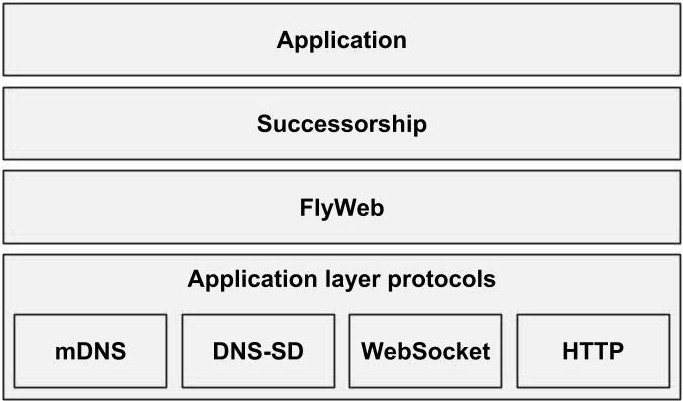
\includegraphics[keepaspectratio,width=6cm]{stack}
    \caption{Successorships Stack}
    \label{fig:stack}
\end{figure}

\noindent\textbf{Roles and shared state.} When a Shippy app is loaded in the browser the new node becomes either a client or server node. 
If it becomes a server node, it becomes a client node to ``itself'' shortly after. 
The application's global state is replicated and shared among all client nodes (see later paragraphs in this section for details). 
The global state can contain arbitrary application data and global metadata accessible only by the \APIshort library. 
One such required metadata field is a \texttt{successors} list containing a list of current clients, except the client node that is currently also the server. 
This list is used to determine which node should become the next server node upon failure of the current one. 
Figure~\ref{fig:roles} depicts the distribution of roles. Node \textit{A} is currently the server with nodes \textit{B...n} being clients. 
Both server and clients have their own replica of the state, accessible through the global state.

\begin{figure}[h]
    \centering
    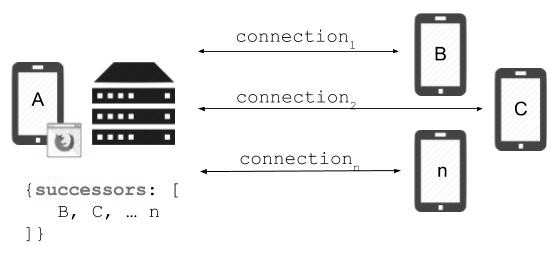
\includegraphics[keepaspectratio,width=6cm]{roles}
    \caption{Successorships Roles}
    \label{fig:roles}
\end{figure}

\noindent\textbf{Service discovery.} 
The \APIshort library comes with a compulsory Firefox add-on responsible for notifying apps with the current set of available \APIshort services. 
In the add-on, we register an event listener to the FlyWeb \textit{DNS-SD} component, which dispatches a list of current local services in frequent intervals.
We sample these events to a maximum frequency of 100ms\footnote{We observed many duplicate and overly frequent event triggers from the \texttt{FlyWebDiscoveryManager} making this sampling necessary.} and filter out all services that were not published in the FlyWeb context\footnote{We aim to filter this list to contain only services published with Shippy rather than FlyWeb in the future, as described in section~\ref{sec:limitations_and_future_work}.}. 
We then dispatch our own events containing the current list of FlyWeb services with the service name, IP address and port on the Browser's global \texttt{window} object. 
These events are then accessible by any \APIshort app.
Listing presents an excerpt of the \APIshort event listener, which is completely transparent to applications using our API.


\begin{lstlisting}[caption={Event listener for service discovery},label={lst:service_discovery}]
window.addEventListener('flywebServicesChanged', function(event) {
    let services = event.detail.services;
    // e.g. [{ serviceName: "QueueApp",
    // serviceUrl: "http://206.12.69.249:51629" }]
});
\end{lstlisting}

\noindent\textbf{Service publication.}
A \APIshort node will publish a service and hereby become a server node in certain cases depending on service discovery events and the current list of successors in the shared state. 
The decision of whether to become a server is first triggered when (1) \textit{the app is loaded} in the browser and there is currently \textit{no service discovered with the app's name}. 
This decision is then repeated (2) any time a \textit{discovery event} occurs and there is \textit{no such service}\footnote{There is one additional requirement to trigger the decision of whether to publish a service when an event reveals there is currently no service for the app: it must have been connected to a server node previously and been disconnected afterwards. 
If this is not the case, the event should not trigger a server publish as this is handled by the first trigger (app load).}. 
In both cases, the node will become a server if \textit{either} of the following conditions is true:
\begin{itemize}
    \item The \texttt successors list is empty \textit{and} this node loaded the application initially\footnote{This is determined by whether the application is currently served by a FlyWeb server node or by other means, e.g. a Web application or a simple HTML file from the file system.}.
    \item The \texttt successors list is not empty \textit{and} the first item in the list refers to itself.
\end{itemize}

If one of the above conditions is met in a decision phase, a service with the app's name will be published and that node will become a server. This will then result in a service advertisement  in the local network using the \textit{mDNS} protocol. 

% Figure~\ref{fig:server} illustrates this behavior.

% \begin{figure}[h]
%     \centering
%     
\includegraphics[keepaspectratio,width=8cm]{server}
%     \caption{Successorships service publication}
%     \label{fig:server}
% \end{figure}


\noindent\textbf{Client connection.}
A \APIshort node will become a client when it discovers a service name/url and connects to it.
To do so, \textit{there must be a \APIshort service running with the app's name} and the \textit{the node is not already connected as a server node}. 
When a node becomes a client, it establishes a \textit{WebSocket} connection to the current server as the first part of the initial handshake. 
On the server side, a unique ID is created for the new client and appended to the \texttt{successors} list. 
The updated \texttt{successors} list is then broadcasted to all currently connected clients. 
The created ID is sent to the new client as the second part of the handshake.
The client node then saves that its ID such that it can be matched against the IDs in the \texttt{successors} list.

\noindent\textbf{Client succession.} 
Whenever the current server fails, a successor must be chosen. 
To do so, clients nodes match their ID against the ones in the \texttt{successors} list.
If their ID matches the first ID in the successor, then that node will become a server node.
Otherwise, it will wait for the new server and connect to it as a client once again.
Considering a server node and clients nodes as depicted in Figure~\ref{fig:roles}, suppose that the server \texttt{A} fails. In this scenario, connected clients \texttt{B} to \texttt{n} detect that failure and match their ID against the ones in the list of successors, as presented in Figure~\ref{fig:succession}. Node \texttt{B} will become a server node as its ID matches the one for the first successor while other nodes will wait and connect to \texttt{B} as clients nodes.

\begin{figure}[h]
    \centering
    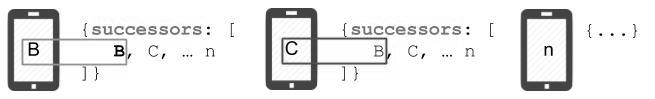
\includegraphics[keepaspectratio,width=6cm]{succession}
    \caption{Successorships client succession}
    \label{fig:succession}
\end{figure}

\noindent\textbf{Server implementation.}
\APIName uses the concept of an in-browser Web server based on the \texttt{navigator.publishServer} implementation in FlyWeb\footnote{https://github.com/flyweb/spec}.
This implementation provides an API for received \textit{HTTP GET} requests and \textit{WebSocket} messages.
Since any Web application relies on static resources (e.g. js, css, images) our FlyWeb server implementation must be able to load and serve these resources when requested by clients.
The documentation of FlyWeb\footnote{https://flyweb.github.io/posts/2016/11/01/introducing-flyweb.html, accessed 2017-12-09} describes that this can be achieved using browser's \textit{Fetch API}\footnote{https://developer.mozilla.org/en-US/docs/Web/API/Fetch\_API, accessed 2017-12-09}.
However, this is essentially just a redirect to the Web app that served the FlyWeb app at the first place.
Since, after a failure, the original Web app and its static resources will not be available to clients that took over the server role from another node \APIshort must store static resources at every node\footnote{Also, we want to support scenarios where only the first client has access to the original Web app that bootstraps the FlyWeb application and clients subsequently only need access to the node that became the first FlyWeb server.}.
We solved this problem by storing all resources required for the \APIshort app in the browser's \texttt{sessionStorage}\footnote{https://developer.mozilla.org/de/docs/Web/API/Window/sessionStorage, accessed 2017-12-09.} that is persistent for the duration of the current browser session.
In the current implementation, all resources obtained upon load of the app are scanned for referenced resources.
These are then fetched\footnote{In the future we aim to omit these secondary requests with a strategy of accessing these resources from the browser's native storage (see section~\ref{sec:limitations_and_future_work}).} and stored in \texttt{sessionStorage}.
Subsequently, when \APIshort request static resources, these can be simply obtained from \texttt{sessionStorage} and served without any access to the original Web app.



% using the \texttt{window.navigator.publishServer} method provided by FlyWeb\footnote{https://github.com/flyweb/spec}. 